% The region under y = x^2 for 0 <= x <= 3 (area 9).
\documentclass[border=4pt]{standalone}
\usepackage{tikz}
\begin{document}
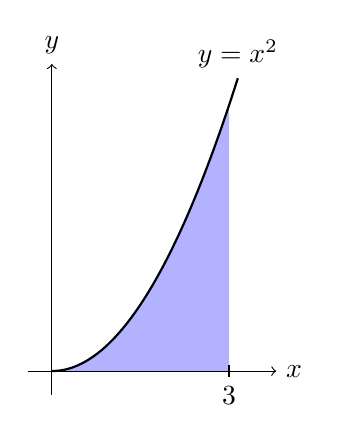
\begin{tikzpicture}[scale=0.75]
  \fill[blue!30] (0,0) -- plot[domain=0:3, samples=60] (\x, {\x*\x/2}) -- (3,0) -- cycle;
  \draw[->] (-0.4,0) -- (3.8,0) node[right] {$x$};
  \draw[->] (0,-0.4) -- (0,5.2) node[above] {$y$};
  \draw[thick] plot[domain=0:3.15, samples=60] (\x, {\x*\x/2}) node[above] {$y=x^2$};
  \draw (3,0.1) -- (3,-0.1) node[below] {$3$};
\end{tikzpicture}
\end{document}
